\documentclass[conference]{IEEEtran}
\ifCLASSINFOpdf
\usepackage[pdftex]{graphicx}
\else
\fi
\usepackage{hyperref}
\hypersetup{
    colorlinks=true,
    linkcolor=blue,
    filecolor=magenta,      
    urlcolor=blue,
}

\urlstyle{same}
% correct bad hyphenation here
\hyphenation{op-tical net-works semi-conduc-tor}
\usepackage{amsmath}
\usepackage[section]{placeins}
\usepackage[font=footnotesize]{caption}
\usepackage{float}

\begin{document}
\title{Movies' IMDb Rating Prediction}
\author{\IEEEauthorblockN{Advait Lonkar}
\IEEEauthorblockA{IMT2017002\\International Institute of Information\\ Technology, Bangalore}
\and
\IEEEauthorblockN{Gandharv Suri}
\IEEEauthorblockA{IMT2017017\\International Institute of Information\\ Technology, Bangalore}
\and
\IEEEauthorblockN{Mili Goyal}
\IEEEauthorblockA{IMT2017513\\International Institute of Information\\ Technology, Bangalore}
}
\maketitle
\begin{abstract}
One simple, but an effective way to determine if a movie is worth watching is to use its IMDb rating. The IMDb top 250 list is, despite the subjective nature of the matter, the list of best movies one can watch. We present a machine learning model to predict the IMDb rating of a movie based on various features provided in the dataset.

\textit{Keywords : IMDb rating, numerical features, }
\end{abstract}
\section{Introduction}
IMDb (Internet Movie Database) is an online database of information related to films, television programs, home videos, video games, and streaming content online – including cast, production crew and personal biographies, plot summaries, trivia, fan and critical reviews, and ratings \cite{IMDB}.\\
IMDb registered users can cast a vote (from 1 to 10) on every released title in the database. Individual votes are then aggregated and summarized as a single IMDb rating, visible on the title’s main page \cite{rating}.\\
The IMDb ratings are accurately calculated using a consistent, unbiased formula, but by no means are these ratings qualitatively \textit{accurate}. An argument can be made that the ratings are too simplistic, which is quite fair : millions of users rate an artistic expression and reduce it into a range of 1 to 10, so obviously some of the nuances of what makes a movie good are lost. \\
But more often than not, people visit IMDb to rate the latest movie they had watched, check ratings of other movies, make watch lists accordingly, and many other such activities. Though the rating is only a number, it can be very informative and useful in itself. A rating cast by thousands of viewers generally represents a well-aggregated rating of a movie. \\
The goal of the project is to predict the IMDb rating of a movie provided various features in the dataset.\\
\section{Problem Statement}
Given various data-points of a movie, predict the IMDb rating of the movie in the range of 1 to 10.\\
This problem falls under the domain of \textbf{Linear Regression}.\\
The evaluation metrics of the presented model will be the variance, standard deviation, root-mean-square-error of the predicted IMDb ratings v/s the actual IMDb rating of a particular movie.\\
\newpage
\section{Data}
\subsection{Data Description}
We have a dataset of 5,043 samples which will later be split into training and testing sets. The dataset was taken from Kaggle \cite{data}.\\
The dataset consists of the following fields:
\begin{itemize}
	\item \textbf{color} : a string field which identifies the color of the movie, color or black and white.
	\item \textbf{director$\_$name} : a string field which identifies the director of the movie.
	\item \textbf{num$\_$critic$\_$for$\_$reviews} : a numeric field which identifies the number of critic reviewers of a movie.
	\item \textbf{duration} : a numeric field which identifies the duration of the movie.
	\item \textbf{director$\_$facebook$\_$likes} : a numeric field which identifies the number of likes on facebook for the director of the movie.
	\item \textbf{actor$\_$3$\_$facebook$\_$likes} : a numeric field which identifies the number of likes on facebook of the 3rd actor of the movie.
	\item \textbf{actor$\_$2$\_$name} : a string field which identifies the name of the 2nd actor of the movie.
	\item \textbf{actor$\_$1$\_$facebook$\_$likes} : a numeric field which identifies the number of likes on facebook of the 1st actor of the movie.
	\item \textbf{gross} : a numeric field which identifies the gross revenue of the movie. 
	\item \textbf{genres}  : a string field which identifies the genre of the movie. 
	\item \textbf{actor$\_$1$\_$name} : a string field which identifies the name of the 1st actor of the movie.
	\item \textbf{movie$\_$title} : a string field which identifies the title of the movie.
	\item \textbf{num$\_$voted$\_$users} : a numeric field which identifies the number of users who voted for the movie. 
	\item \textbf{cast$\_$total$\_$facebook$\_$likes} : a numeric field which identifies the number of likes on facebook of the cast of the movie.
	\item \textbf{actor$\_$3$\_$name} : a string field which identifies the name of the 3rd actor of the movie.
	\item \textbf{facenumber$\_$in$\_$poster} : a numeric field which identifies the number of faces in the poster of the movie.
	\item \textbf{plot$\_$keywords}  : a string field which identifies the plot keywords of the movie.
	\item \textbf{movie$\_$imdb$\_$link} : a string field which identifies the imdb link of the movie. 
	\item \textbf{num$\_$user$\_$for$\_$reviews} : a numeric field which identifies the number of user for reviews of the movie. 
	\item \textbf{language}  : a string field which identifies the language of the movie.
	\item \textbf{country}  : a string field which identifies the country of the movie.
	\item \textbf{content$\_$rating} : a string field which identifies the conten rating (R or PG-13) of the movie.
	\item \textbf{budget} : a numeric field which identifies the budget of the movie.
	\item \textbf{title$\_$year} : a numeric field which identifies the year of release of the movie. 
	\item \textbf{actor$\_$2$\_$facebook$\_$likes} : a numeric field which identifies the number of likes on facebook of the 2nd actor of the movie.
	\item \textbf{imdb$\_$score} : a numeric field which identifies the imdb score of the movie.
	\item \textbf{aspect$\_$ratio}  : a numeric field which identifies the aspect ratio of the movie. 
	\item \textbf{movie$\_$facebook$\_$likes}  : a numeric field which identifies the number of likes on facebook of the movie.\\
\end{itemize}
\subsection{Data Exploration and Visualization}


% Label frequency
\begin{figure}[H]
  \centering	
  \captionsetup{justification=centering}
  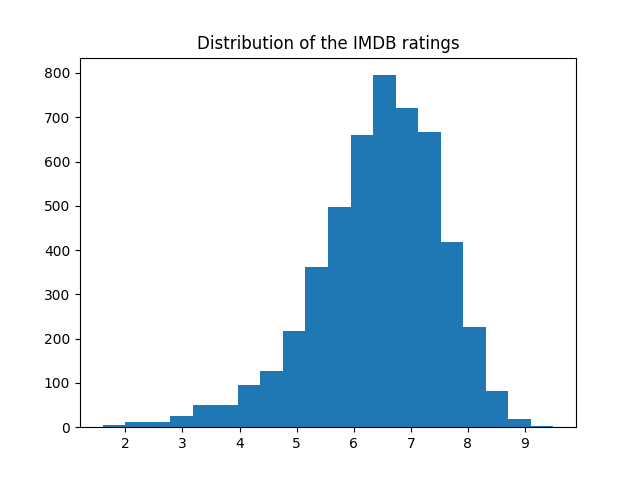
\includegraphics[height=6cm, width=9cm, trim={0mm 0mm 0mm 0mm},clip]{../visualizations/IMDB-Score-Histogram}
  \caption{IMDB-Score histogram}
  \label{fig:fig1}
\end{figure}

\section{Pre-Processing}
\subsection{Dropping rows}
The columns $gross$ and $budget$ had the maximum number of missing values, 884 and 492 respectively. Imputation of so many values would provide faulty results, so we decided to drop the rows corressponding to the missing fields of columns $gross$ and $budget$.
\subsection{Dropping columns}
	\begin{enumerate}
		\item $aspect\_ratio$ : The two most frequent values of $aspect\_ratio			$ and the rest of the $aspect\_ratio$ values had similar mean IMDb 				ratings, i.e. the aspect ratio values did not have any significant effect on the IMDb ratings. So we dropped the column $aspect\_ratio$.
		\item $language$ : Most of the movies (more than 90$\%$) are in 				English, so we dropped the column $language$.
		\item $color$ : Most of the movies are colored (more than 90$\%$), so 			we dropped the column $color$.
		\item $plot\_keywords, director\_name, actor\_1\_name, actor\_2\_name,			\\ actor\_3\_name, genres, movie\_imdb\_link$ : Most of the values in 			these fields are unique, so we dropped all of these columns.
	\end{enumerate}
\subsection{Labelling}
The $country$ column had over 79$\%$ of values as USA and 8$\%$ as UK. So we labelled all the other countries as $Others$.


\section{Feature Extraction}
\section{Model Building}
\newpage
\bibliographystyle{unsrt}
\bibliography{Bibliography}
\end{document}